\chapter{C\`{a}lculs B\`{a}sics}\label{sec:calc_bas}

\section{Introducci\'{o}}
Es tracten en aquest cap\'{\i}tol c\`{a}lculs b\`{a}sics que poden utilitzar-se en la
resoluci\'{o} de diversos problemes electrot\`{e}cnics.



\section{C\`{a}lculs en per unitat} \label{sec:seccio_pu} \index{pu}\index{per unitat}

Les magnituds expressades en {"<}pu{">} (per unitat) s\'{o}n \'{u}tils quan es treballa
amb xarxes de corrent altern on hi ha transformadors, i per tant m\'{e}s d'un nivell de tensi\'{o}.

\subsection{M\`{e}tode de c\`{a}lcul} \index{pu!m\`{e}tode de c\`{a}lcul}

\index{pu!magnituds base fonamentals} El primer pas consisteix a
escollir unes magnituds base. Les magnituds base fonamentals s\'{o}n la
pot\`{e}ncia i la tensi\'{o}; s'escull una pot\`{e}ncia base $S\ped{B}$ per a
tota la xarxa, i tantes tensions base com nivells de tensi\'{o}
diferents tingui la xarxa $U_{\text{B}_1}, U_{\text{B}_2}, \ldots,
U_{\text{B}_n}$:
\begin{equation}
   \text{Magnituds base fonamentals}\;\left\{
\begin{array}{l}
   S\ped{B} \\
   U_{\text{B}_1}, U_{\text{B}_2}, \ldots, U_{\text{B}_n}
\end{array}
\right.
\end{equation}

Normalment s'escull com a tensions base les tensions nominals dels transformadors de la
xarxa, i com a pot\`{e}ncia base la potencia nominal d'un del transformadors o generadors de la xarxa; tamb\'{e} \'{e}s usual utilitzar com a pot\`{e}ncia base el valor 100\unit{MVA}.

En el cas de circuits monof\`{a}sics, les tensions base s\'{o}n les tensions monof\`{a}siques, o fase--neutre $U\ped{FN}$, i la pot\`{e}ncia base \'{e}s la potencia monof\`{a}sica $S\ped{1F}$. En el cas de circuits trif\`{a}sics, podem escollir com a tensions base les tensions fase--neutre $U\ped{FN}$ i com a pot\`{e}ncia base la pot\`{e}ncia  monof\`{a}sica $S\ped{1F}$, o b\'{e} podem escollir com a tensions base les tensions fase--fase $U\ped{FF}$ i com a pot\`{e}ncia base la potencia trif\`{a}sica $S\ped{3F}$.

\index{pu!magnituds base}A partir de la pot\`{e}ncia base i de les tensions base es
defineixen els corrents base $I_{\text{B}_i}$, les imped\`{a}ncies base $Z_{\text{B}_i}$ i les
admit\`{a}ncies base $Y_{\text{B}_i}$. Segons que s'utilitzin les tensions i pot\`{e}ncies monof\`{a}siques o trif\`{a}siques com a magnituds base, tenim:
\begin{equation}
\begin{array}{c}  S\ped{B}=S\ped{1F} \\ U_{\text{B}_i} = U_{\text{FN}_i} \\ (i=1,\ldots,n) \end{array}
\left\{
\begin{array}{lll}
   I_{\text{B}_i} &= &\dfrac{S\ped{B}}{U_{\text{B}_i}} \\[2.5ex]
   Z_{\text{B}_i} &= &\dfrac{U_{\text{B}_i}^2}{S\ped{B}} = \dfrac{U_{\text{B}_i}}{I_{\text{B}_i}} \\[2.5ex]
   Y_{\text{B}_i} &= &\dfrac{S\ped{B}}{U_{\text{B}_i}^2} = \dfrac{I_{\text{B}_i}}{U_{\text{B}_i}}
\end{array}
\right.
\qquad\qquad
\begin{array}{c} S\ped{B}=S\ped{3F} \\ U_{\text{B}_i} = U_{\text{FF}_i} \\ (i=1,\ldots,n) \end{array}
\left\{
\begin{array}{lll}
   I_{\text{B}_i} &= &\dfrac{S\ped{B}}{\sqrt{3} U_{\text{B}_i}} \\[2.5ex]
   Z_{\text{B}_i} &= &\dfrac{U_{\text{B}_i}^2}{S\ped{B}}= \dfrac{U_{\text{B}_i}}{\sqrt{3} I_{\text{B}_i}} \\[2.5ex]
   Y_{\text{B}_i} &= &\dfrac{S\ped{B}}{U_{\text{B}_i}^2} = \dfrac{\sqrt{3} I_{\text{B}_i}}{U_{\text{B}_i}}
\end{array}
\right.
\label{eq:bases_pu}
\end{equation}

Les magnituds expressades en per unitat (escrites usualment en min\'{u}scules) s'obtenen
dividint les magnituds reals (escrites usualment en maj\'{u}scules) pels valors base corresponents:
\begin{equation}
   \cmplx{s} = \frac{\cmplx{S}}{S\ped{B}} \qquad \cmplx{u} = \frac{\cmplx{U}}{U\ped{B}} \qquad \cmplx{i} = \frac{\cmplx{I}}{I\ped{B}} \qquad \cmplx{z} = \frac{\cmplx{Z}}{Z\ped{B}} \qquad \cmplx{y} = \frac{\cmplx{Y}}{Y\ped{B}}
\end{equation}

Quan es tracta de resoldre circuits trif\`{a}sics equilibrats fem servir sempre els circuits equivalents per fase, i podem escollir aleshores com a valors base per a la pot\`{e}ncia i la tensi\'{o}, la pot\`{e}ncia monof\`{a}sica $S\ped{1F}$ i la tensi\'{o} fase--neutre $U\ped{FN}$ respectivament, o la pot\`{e}ncia trif\`{a}sica $S\ped{3F}$ i la tensi\'{o} fase--fase $U\ped{FF}$ respectivament.


 Quan fem la reducci\'{o} de valors reals a valors en per unitat, hem de ser conseq\"{u}ents i utilitzar sempre les pot\`{e}ncies monof\`{a}siques i les tensions fase-neutre en el primer cas, i les pot\`{e}ncies trif\`{a}siques i les tensions fase-fase en el segon cas.

 Donat que es verifica $S\ped{3F}=3 S\ped{1F}$ i $U\ped{FF}=\sqrt{3}U\ped{FN}$, els valors  del corrent base $I\ped{B}$, de la imped\`{a}ncia base $Z\ped{B}$ i  de l'admit\`{a}ncia base $Y\ped{B}$ s\'{o}n els mateixos, tan si utilitzem $S\ped{B}=S\ped{1F}$ i $U\ped{B}=U\ped{FN}$, con si utilitzem $S\ped{B}=S\ped{3F}$ i $U\ped{B}=U\ped{FF}$.

 En ambd\'{o}s casos $I\ped{B}$ i $\cmplx{I}$ s\'{o}n corrents fase--neutre, $Z\ped{B}$ i $\cmplx{Z}$ s\'{o}n imped\`{a}ncies fase--neutre i $Y\ped{B}$ i $\cmplx{Y}$ s\'{o}n admit\`{a}ncies fase--neutre; si tenim c\`{a}rregues connectades en triangle, cal transformar-les en c\`{a}rregues equivalents connectades en estrella per tal de poder aplicar aquest m\`{e}tode (vegeu la secci\'{o} \ref{secc:d_y}).

El pas seg\"{u}ent consisteix a representar el circuit equivalent en
per unitat i resoldre'l; en el cas de circuits trif\`{a}sics, i com a conseq\"{u}\`{e}ncia del proc\'{e}s utilitzat, el circuit equivalent en per unitat \'{e}s un circuit monof\`{a}sic i com a tal l'hem de resoldre, \'{e}s a dir, sense la intervenci\'{o} del factor $\sqrt{3}$.

Un cop resolt el circuit, es multipliquen les magnituds obtingudes en per unitat pels
seus valors base respectius, per tal d'obtenir les magnituds reals:
\begin{equation}
   \cmplx{S} = \cmplx{s} S\ped{B} \qquad \cmplx{U} = \cmplx{u} U\ped{B} \qquad \cmplx{I} = \cmplx{i} I\ped{B} \qquad \cmplx{Z} = \cmplx{z} Z\ped{B} \qquad \cmplx{Y} = \cmplx{y} Y\ped{B}
\end{equation}

\subsection{Canvi de base}\label{sec:canvi-base} \index{pu!canvi de base}

Normalment les imped\`{a}ncies de transformadors (imped\`{a}ncia de curtcircuit) o de generadors (imped\`{a}ncia sincr\`{o}nica, transit\`{o}ria, etc.) estan referides a les magnituds nominals de la m\`{a}quina en q\"{u}esti\'{o}.


Si les magnituds base escollides coincideixen amb les nominals de la m\`{a}quina,
la imped\`{a}ncia de la m\`{a}quina en q\"{u}esti\'{o} estar\`{a} expressada ja directament en per unitat.

 En canvi si les magnituds base s\'{o}n diferents de les nominals de la m\`{a}quina, caldr\`{a} fer un canvi de base per tal de referir la imped\`{a}ncia de la m\`{a}quina a les magnituds base escollides.

De forma gen\`{e}rica, si $\cmplx{z}$ \'{e}s una imped\`{a}ncia referida a la base $U\ped{B}$ i $S\ped{B}$, podem obtenir la imped\`{a}ncia $\cmplx{z}'$ referida a la base $U_{\text{B}'}$ i $S_{\text{B}'}$, mitjan\c{c}ant el canvi:
\begin{equation}
   \cmplx{z}' = \cmplx{z} \; \frac{Z\ped{B}}{Z\ped{B}'} = \cmplx{z} \; \frac{U\ped{B}^2}{U_{\text{B}'}^2} \; \frac{S_{\text{B}'}}{S\ped{B}}\label{eq_pu_canvi_base}
\end{equation}

\begin{exemple}[Aplicaci\'{o} del m\`{e}tode de c\`{a}lcul en per unitat]
    Es tracte de calcular el corrent de curtcircuit trif\`{a}sic en el punt F de la xarxa seg\"{u}ent, suposant
    que el sistema est\`{a} treballant en buit.
    \begin{center}
        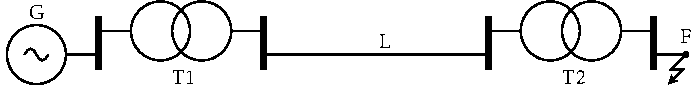
\includegraphics{Imatges/Cap-Fonaments-pu-Circuit1.pdf}
    \end{center}

    Les dades del generador G, del transformador T1, de la l\'{\i}nia L i del transformador T2 s\'{o}n:
    \begin{align*}
       S\ped{G} &= \SI{60}{MVA} & S\ped{T1} &= \SI{40}{MVA} & l\ped{L} &= \SI{22}{km} & S\ped{T2} &=
       \SI{12}{MVA} \\
       U\ped{G} &= \SI{10,5}{kV} & m\ped{T1} &= \SI{10,5}{kV}\!:\!\SI{63}{kV} & U\ped{L} &= \SI{60}{kV} & m\ped{T2} &= \SI{60}{kV}\!:\!\SI{10,5}{kV} \\
       X''\ped{G} &= \SI{12}{\%} & X\ped{T1} &= \SI{10}{\%} & X\ped{L} &= \SI{0,4}{\ohm/km} & X\ped{T2} &= \SI{8}{\%}
    \end{align*}

    Escollim en primer lloc les seg\"{u}ents magnituds base: $S\ped{B} = \SI{60}{MVA}$ i $U\ped{B}
    = \SI{10,5}{kV} / \SI{63}{kV} / \SI{10,5}{kV}$.

    Calculem a continuaci\'{o} els valors en per unitat dels diferents elements de la xarxa:

    \textbf{Generador}. En coincidir les magnituds base amb les nominals del generador tenim
     directament:
    \[
    x''\ped{G} = \SI{0,12}{pu}
    \]

    \textbf{Transformador 1}. La relaci\'{o} de transformaci\'{o} i la react\`{a}ncia s\'{o}n respectivament:
    \begin{align*}
    m\ped{T1} &= \frac{\SI{10,5}{kV}}{\SI{10,5}{kV}} :
    \frac{\SI{63}{kV}}{\SI{63}{kV}} = 1\!:\!1 \\[3mm]
    x\ped{T1} &= \num{0,10} \times \frac{(\SI{63}{kV})^2}{(\SI{63}{kV})^2} \times
    \frac{\SI{60}{MVA}}{\SI{40}{MVA}}  = \SI{0,15}{pu}
    \end{align*}

    \textbf{L\'{\i}nia}. La react\`{a}ncia \'{e}s:
    \[
    x\ped{L} = \frac{\SI{0,4}{\ohm/km} \times \SI{22}{km}} {(\SI{63}{kV})^2/\SI{60}{MVA}}  =
    \SI{0,1330}{pu}
    \]

    \textbf{Transformador 2}. La relaci\'{o} de transformaci\'{o} i la react\`{a}ncia s\'{o}n respectivament:
    \begin{align*}
    m\ped{T2} &= \frac{\SI{60}{kV}}{\SI{63}{kV}} :
    \frac{\SI{10,5}{kV}}{\SI{10,5}{kV}} = \num{0,9524}\!:\!1 \\[3mm]
    x\ped{T2} &= \num{0,08} \times \frac{(\SI{10,5}{kV})^2}{(\SI{10,5}{kV})^2} \times
    \frac{\SI{60}{MVA}}{\SI{12}{MVA}}  = \SI{0,4}{pu}
    \end{align*}

    \textbf{Tensi\'{o} en el punt F}. La tensi\'{o} abans del curtcircuit \'{e}s la mateixa que la del generador G, elevada pel transformador T1 i redu\"{\i}da despr\'{e}s pel transformador T2:
    \[
    \cmplx{u}\ped{F} = \frac{\SI{10,5}{kV} \times
    \dfrac{\SI{63}{kV}}{\SI{10,5}{kV}} \times
    \dfrac{\SI{10,5}{kV}}{\SI{60}{kV}}}{\SI{10,5}{kV}} = \SI{1,05}{pu}
    \]

    A partir d'aquests valors calculats, tenim el seg\"{u}ent circuit equivalent en per unitat, durant el
    curtcircuit en el punt F:

    \begin{center}
       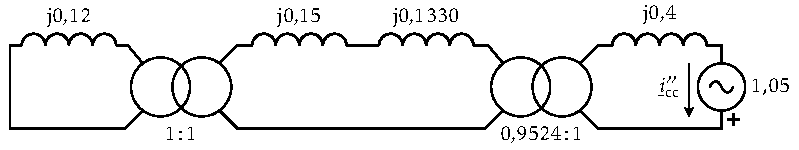
\includegraphics{Imatges/Cap-Fonaments-pu-Circuit2.pdf}
    \end{center}

    El corrent de curtcircuit buscat val:
    \begin{align*}
    |\cmplx{i}''\ped{cc}| &= \left| \frac{\num{1,05}}{\ju \left( \num{0,4} + \frac{\num{0,15} + \num{0,1330}}{\num{0,9524}^2} + \frac{\num{0,12}}{\num{0,9524}^2 \times 1^2} \right)} \right| =
     \SI{1,2436}{pu} \\[3mm]
     |\cmplx{I}''\ped{cc}| &= \SI{1,2436}{pu}\times\frac{\SI{60}{MVA}}{\sqrt{3}\times \SI{10,5}{kV}} =
     \SI{4,1}{kA}
    \end{align*}

     A l'hora de calcular el corrent de curtcircuit utilitzant el circuit equivalent en per unitat,
     s'observa que el transformador T1 \'{e}s com si hagu\'{e}s desaparegut,
     aix\`{o} \'{e}s aix\'{\i}, ja que la seva relaci\'{o} de transformaci\'{o} ha esdevingut
     $1\!:\!1$, en coincidir les tensions base amb les seves tensions nominals.

     No passa el mateix amb el transformador T2, ja que no es compleix
     la coincid\`{e}ncia entre les seves tensions nominals i les tensions
     base.

     No obstant, at\`{e}s que l'elecci\'{o} de les tensions base \'{e}s
     arbitr\`{a}ria, si en lloc de \SI{10,5}{kV} com a tercera tensi\'{o} base,
     escollim
     $\frac{\SI{63}{kV}}{\SI{60}{kV} / \SI{10,5}{kV}}=\SI{11,025}{kV}$,
     tindrem:
    \begin{align*}
       m\ped{T2} &= \frac{60\unit{kV}}{63\unit{kV}} : \frac{\SI{10,5}{kV}}{\SI{11,025}{kV}}
       = \num{0,9524}\!:\!\num{0,9524} = 1\!:\!1 \\[3mm]
       x\ped{T2} &= \num{0,08} \times \frac{(\SI{10,5}{kV})^2}{(\SI{11,025}{kV})^2 } \times
       \frac{60\unit{MVA}}{12\unit{MVA}}  = \SI{0,3628}{pu}\\[3mm]
       \cmplx{u}\ped{F} &= \frac{\SI{10,5}{kV} \times \dfrac{63\unit{kV}}{\SI{10,5}{kV}} \times
       \dfrac{\SI{10,5}{kV}}{60\unit{kV}}}{\SI{11,025}{kV}} = 1\unit{pu}
    \end{align*}

    Utilitzant aquests nous valors, podem prescindir totalment dels dos
    transformadors, i calcular el corrent de curtcircuit utilitzant
    l'expressi\'{o} seg\"{u}ent:
    \begin{align*}
    |\cmplx{i}''\ped{cc}| &= \left| \frac{1}{\ju ( \num{0,3628} + \num{0,15} +
    \num{0,1330} + \num{0,12} )} \right| = \SI{1,3058}{pu} \\[3mm]
    |\cmplx{I}''\ped{cc}| &=
    \SI{1,3058}{pu}\times\frac{60\unit{MVA}}{\sqrt{3}\times \SI{11,025}{kV}} =
    \SI{4,1}{kA}
    \end{align*}

    Evidentment, el valor final \'{e}s el mateix independentment de quines
    siguin les tensions base escollides.
\end{exemple}

\subsection{Valors base per a branques que treballen a diferent tensi\'{o}, amb acoblament magn\`{e}tic}\index{pu!acoblament magn\`{e}tic}

En la figura \vref{pic:pu_zm} hi ha representades dues branques acoblades magn\`{e}ticament; es fa el sup\`{o}sit addicional que les tensions de treball de les dues branques s\'{o}n diferents.

\begin{center}
    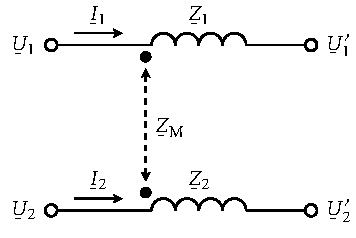
\includegraphics{Imatges/Cap-Fonaments-pu-ZM.pdf}
    \captionof{figure}{Valors base en un acoblament magn\`{e}tic}
    \label{pic:pu_zm}
\end{center}

Les equacions que relacionen els corrents i les tensions d'aquest circuit s\'{o}n:
\begin{subequations}
\begin{align}
    \cmplx{U}_1 - \cmplx{U}'_1 &= \cmplx{Z}_1 \cmplx{I}_1 + \cmplx{Z}\ped{M} \cmplx{I}_2   \\[2mm]
    \cmplx{U}_2 - \cmplx{U}'_2 &= \cmplx{Z}_2 \cmplx{I}_2 + \cmplx{Z}\ped{M} \cmplx{I}_1
\end{align}
\end{subequations}

Si volem convertir aquestes magnituds a valors en per unitat, hem d'escollir  una potencia base $S\ped{B}$ i dues tensions base, una  per a cada branca, $U_{\text{B}_1}$ i  $U_{\text{B}_2}$, i a partir de les equacions \eqref{eq:bases_pu} obtenir els corrents, imped\`{a}ncies i admit\`{a}ncies base per a cada branca.

De la mateixa manera que s'ha dit en els apartats anteriors, en el cas de circuits trif\`{a}sics, podem escollir com a tensions base les tensions fase--neutre $U\ped{FN}$ i com a pot\`{e}ncia base la pot\`{e}ncia  monof\`{a}sica $S\ped{1F}$, o b\'{e} podem escollir com a tensions base les tensions fase--fase $U\ped{FF}$ i com a pot\`{e}ncia base la potencia trif\`{a}sica $S\ped{3F}$.


Per tal de calcular la imped\`{a}ncia base $Z_{\text{B}_\text{M}}$ per convertir $\cmplx{Z}\ped{M}$ en un valor en per unitat, no podem utilitzar les equacions \eqref{eq:bases_pu}, ja que cadascuna de les dues branques de l'acoblament magn\`{e}tic est\`{a} a una tensi\'{o} diferent; en aquest cas, cal utilitzar l'equaci\'{o} que es por trobar en \cite{TLE}:
\begin{equation}
    Z_{\text{B}_\text{M}} = \frac{U_{\text{B}_1} U_{\text{B}_2}} {S\ped{B}}
\end{equation}

El valor en per unitat $\cmplx{z}\ped{M}$ corresponent a $\cmplx{Z}\ped{M}$ s'obt\'{e} de la manera usual:
\begin{equation}
    \cmplx{z}\ped{M} = \frac{\cmplx{Z}\ped{M}}{Z_{\text{B}_\text{M}}}
\end{equation}


\subsection{Valors base per a branques que treballen a diferent tensi\'{o}, amb acoblament capacitiu}\index{pu!acoblament capacitiu}

En la figura \vref{pic:pu_ym} hi ha representades dues branques acoblades capacitivament; es fa el sup\`{o}sit addicional que les tensions de treball de les dues branques s\'{o}n diferents.

\begin{center}
    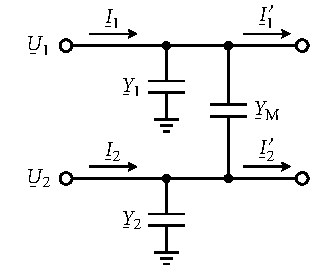
\includegraphics{Imatges/Cap-Fonaments-pu-YM.pdf}
    \captionof{figure}{Valors base en un acoblament capacitiu}
    \label{pic:pu_ym}
\end{center}

Les equacions que relacionen els corrents i les tensions d'aquest circuit s\'{o}n:
\begin{subequations}
\begin{align}
    \cmplx{I}_1  &= \cmplx{Y}_1 \cmplx{U}_1 +  \cmplx{Y}\ped{M}(\cmplx{U}_1-\cmplx{U}_2)  + \cmplx{I}'_1   \\[2mm]
    \cmplx{I}_2  &= \cmplx{Y}_2 \cmplx{U}_2 +  \cmplx{Y}\ped{M}(\cmplx{U}_2-\cmplx{U}_1)  + \cmplx{I}'_2
\end{align}
\end{subequations}

Si volem convertir aquestes magnituds a valors en per unitat, hem d'escollir  una potencia base $S\ped{B}$ i dues tensions base, una  per a cada branca, $U_{\text{B}_1}$ i  $U_{\text{B}_2}$, i a partir de les equacions \eqref{eq:bases_pu} obtenir els corrents, imped\`{a}ncies i admit\`{a}ncies base per a cada branca.

De la mateixa manera que s'ha dit en els apartats anteriors, en el cas de circuits trif\`{a}sics, podem escollir com a tensions base les tensions fase--neutre $U\ped{FN}$ i com a pot\`{e}ncia base la pot\`{e}ncia  monof\`{a}sica $S\ped{1F}$, o b\'{e} podem escollir com a tensions base les tensions fase--fase $U\ped{FF}$ i com a pot\`{e}ncia base la potencia trif\`{a}sica $S\ped{3F}$.


Per tal de  calcular l'admit\`{a}ncia base $Y_{\text{B}_\text{M}}$ per convertir $\cmplx{Y}\ped{M}$ en un valor en per unitat, no podem utilitzar les equacions \eqref{eq:bases_pu}, ja que cadascuna de les dues branques de l'acoblament capacitiu est\`{a} a una tensi\'{o} diferent; en aquest cas, cal utilitzar l'equaci\'{o} que es por trobar en \cite{TLE}:
\begin{equation}
    Y_{\text{B}_\text{M}} = \frac{S\ped{B}}{U_{\text{B}_1} U_{\text{B}_2}}
\end{equation}

El valor en per unitat\ $\cmplx{y}\ped{M}$ corresponent a $\cmplx{Y}\ped{M}$ s'obt\'{e} de la manera usual:
\begin{equation}
    \cmplx{y}\ped{M} = \frac{\cmplx{Y}\ped{M}}{Y_{\text{B}_\text{M}}}
\end{equation}


\section{Circuits divisors de tensi\'{o} i divisors de corrent}\label{sec:div_tens_corr}

Un circuit divisor de tensi\'{o} est\`{a} format per un conjunt
d'imped\`{a}ncies en s\`{e}rie, i el que es pret\'{e}n \'{e}s calcular la caiguda de
tensi\'{o} en cada imped\`{a}ncia, en funci\'{o} de la caiguda de tensi\'{o} total.

Un circuit divisor de corrent, en canvi, est\`{a} format per un conjunt
d'imped\`{a}ncies en para{\l.l}el, i el que es pret\'{e}n \'{e}s calcular el
corrent que circula per cada imped\`{a}ncia, en funci\'{o} del corrent
total.

\subsection{Circuits divisors de tensi\'{o}}\index{circuits divisors!de
tensi\'{o}}

En la Figura \vref{pic:div_tensio} es pot veure un circuit divisor
de tensi\'{o}, pel qual es vol calcular la caiguda de tensi\'{o}
$\cmplx{U}_i$ en la imped\`{a}ncia $\cmplx{Z}_i$, a partir de la caiguda
de tensi\'{o} total $\cmplx{U}\ped{total}$.

\begin{center}
\centering
    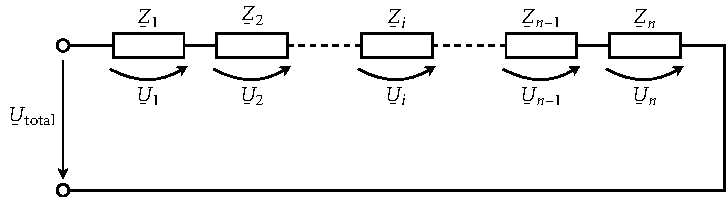
\includegraphics{Imatges/Cap-Fonaments-Divisor-Tensio.pdf}
    \captionof{figure}{Circuit divisor de tensi\'{o}}
    \label{pic:div_tensio}
\end{center}

La imped\`{a}ncia total $\cmplx{Z}\ped{total}$ del circuit val:
\begin{equation}
    \cmplx{Z}\ped{total} = \sum_{i=1}^n \cmplx{Z}_i
\end{equation}

Utilitzant aquest valor, la tensi\'{o} $\cmplx{U}_i$ val:
\begin{equation}
    \cmplx{U}_i = \frac{\cmplx{Z}_i}{\cmplx{Z}\ped{total}}\,\cmplx{U}\ped{total}\qquad (i=1,\dots,n)\label{eq:div_tensio}
\end{equation}

\subsection{Circuits divisors de corrent}\index{circuits divisors!de
corrent}

En la Figura \vref{pic:div_corrent} es pot veure un circuit divisor
de corrent, pel qual es vol calcular el corrent $\cmplx{I}_i$ que
circula per la imped\`{a}ncia $\cmplx{Z}_i$, a partir del corrent total
$\cmplx{I}\ped{total}$.
\begin{center}
\centering
    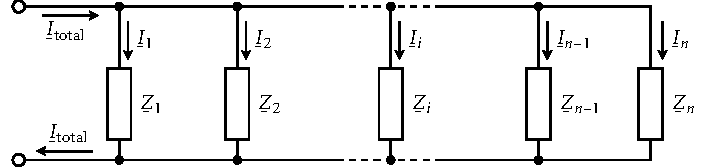
\includegraphics{Imatges/Cap-Fonaments-Divisor-Corrent.pdf}
    \captionof{figure}{Circuit divisor de corrent}
    \label{pic:div_corrent}
\end{center}

La imped\`{a}ncia total $\cmplx{Z}\ped{total}$ del circuit val:
\begin{equation}
    \cmplx{Z}\ped{total} = \frac{1}{\displaystyle\sum_{i=1}^n \frac{1}{\cmplx{Z}_i}}
\end{equation}

Utilitzant aquest valor, el corrent $\cmplx{I}_i$ val:
\begin{equation}
    \cmplx{I}_i = \frac{\cmplx{Z}\ped{total}}{\cmplx{Z}_i}\,\cmplx{I}\ped{total} \qquad (i=1,\dots,n)\label{eq:div_corrent}
\end{equation}




\section{\texorpdfstring{Transformaci\'{o} estrella $\boldsymbol{\leftrightarrow}$ triangle d'imped\`{a}ncies}
    {Transformaci\'{o} estrella-triangle d'imped\`{a}ncies}}\label{secc:d_y} \index{transformaci\'{o}
estrella $\leftrightarrow$ triangle}

En un sistema trif\`{a}sic, pot interessar transformar tres imped\`{a}ncies connectades en
estrella en tres imped\`{a}ncies equivalents connectades en triangle
$(\text{Y}\rightarrow\Delta)$, o a l'inrev\'{e}s, transformar tres imped\`{a}ncies connectades en
triangle en tres imped\`{a}ncies equivalents connectades en estrella
$(\Delta\rightarrow\text{Y})$. Atenent a la Figura \vref{pic:Y_D}, tenim les seg\"{u}ents
transformacions:

\begin{equation}\label{eq:Y_D}
   \text{Y}\rightarrow\Delta\;\left\{
   \begin{array}{lll}
      \cmplx{Z}_{\alphaup\betaup} &= &\displaystyle \cmplx{Z}_{\alphaup} + \cmplx{Z}_{\betaup} + \frac{\cmplx{Z}_{\alphaup}\,\cmplx{Z}_{\betaup}}{\cmplx{Z}_{\gammaup}}  \\[2.5ex]
      \cmplx{Z}_{\betaup\gammaup} &= &\displaystyle \cmplx{Z}_{\betaup} + \cmplx{Z}_{\gammaup} + \frac{\cmplx{Z}_{\betaup}\,\cmplx{Z}_{\gammaup}}{\cmplx{Z}_{\alphaup}}  \\[2.5ex]
      \cmplx{Z}_{\gammaup\alphaup} &= &\displaystyle \cmplx{Z}_{\gammaup} + \cmplx{Z}_{\alphaup} + \frac{\cmplx{Z}_{\gammaup}\, \cmplx{Z}_{\alphaup}}{\cmplx{Z}_{\betaup}}
   \end{array}
   \right.
   \qquad\qquad
   \Delta\rightarrow\text{Y}\;\left\{
   \begin{array}{lll}
      \cmplx{Z}_{\alphaup} &= &\dfrac{\cmplx{Z}_{\alphaup\betaup}\, \cmplx{Z}_{\gammaup\alphaup}}{  \cmplx{Z}_{\alphaup\betaup} + \cmplx{Z}_{\betaup\gammaup}+ \cmplx{Z}_{\gammaup\alphaup}}  \\[2.5ex]
      \cmplx{Z}_{\betaup} &= &\dfrac{\cmplx{Z}_{\betaup\gammaup}\, \cmplx{Z}_{\alphaup\betaup}}{  \cmplx{Z}_{\alphaup\betaup} + \cmplx{Z}_{\betaup\gammaup}+ \cmplx{Z}_{\gammaup\alphaup}}  \\[2.5ex]
      \cmplx{Z}_{\gammaup} &= &\dfrac{\cmplx{Z}_{\gammaup\alphaup}\, \cmplx{Z}_{\betaup\gammaup}}{  \cmplx{Z}_{\alphaup\betaup} + \cmplx{Z}_{\betaup\gammaup}+ \cmplx{Z}_{\gammaup\alphaup}}
   \end{array}
   \right.
\end{equation}

\begin{center}
    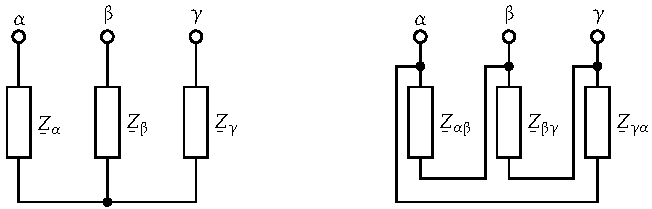
\includegraphics{Imatges/Cap-CalcBas-YD.pdf}
    \captionof{figure}{Transformaci\'{o} estrella $\leftrightarrow$ triangle
d'imped\`{a}ncies}
    \label{pic:Y_D}
\end{center}
\break
\begin{exemple}[Transformaci\'{o} triangle $\rightarrow$ estrella]
    Es vol transformar tres imped\`{a}ncies connectades en triangle, de
    valors $ \cmplx{Z}_{\alphaup\betaup}=\SI{10}{\ohm}$,
    $\cmplx{Z}_{\betaup\gammaup}=\SI{-j10}{\ohm}$ i
    $\cmplx{Z}_{\gammaup\alphaup}=\SI{-j10}{\ohm}$, en tres imped\`{a}ncies
    equivalents connectades en estrella.

    A partir de les equacions \eqref{eq:Y_D}  tenim:
    \begin{align*}
       \cmplx{Z}_{\alphaup} & = \frac{\SI{10}{\ohm}\times(\SI{-j10}{\ohm})}{\SI{10}{\ohm} - \SI{j10}{\ohm} - \SI{j10}{\ohm}} = \SI{4-j2}{\ohm} \\[1.5ex]
       \cmplx{Z}_{\betaup} & = \frac{\SI{-j10}{\ohm}\times \SI{10}{\ohm}}{\SI{10}{\ohm} - \SI{j10}{\ohm} - \SI{j10}{\ohm}} = \SI{4-j2}{\ohm} \\[1.5ex]
    \cmplx{Z}_{\gammaup} &=
    \frac{\SI{-j10}{\ohm}\times(\SI{-j10}{\ohm})}{\SI{10}{\ohm} -
    \SI{j10}{\ohm} - \SI{j10}{\ohm}} = \SI{-2-j4}{\ohm}
    \end{align*}

    \'{E}s possible, com en aquest cas pel que fa a $\cmplx{Z}_{\gammaup}$,
    obtenir un valor amb una part real negativa (resist\`{e}ncia negativa);
    no obstant, encara que no existeixi f\'{\i}sicament aquesta resist\`{e}ncia,
    el seu valor \'{e}s matem\`{a}ticament correcte i es pot utilitzar en
    c\`{a}lculs subseg\"{u}ents.
\end{exemple}



\section{Resoluci\'{o} de circuits coneixent la pot\`{e}ncia absorbida per la
c\`{a}rrega}\label{sec:EZS}

Es tracta en aquest apartat la resoluci\'{o} de circuits simples,
formats per una font de tensi\'{o} en s\`{e}rie amb una imped\`{a}ncia, la qual
alimenta a una c\`{a}rrega; aquesta c\`{a}rrega no est\`{a} definida per la seva
imped\`{a}ncia o admit\`{a}ncia, sin\'{o} per la pot\`{e}ncia que absorbeix\footnote{Aquest \'{e}s un cas particular
del problema del flux de c\`{a}rregues en
sistemes el\`{e}ctrics de pot\`{e}ncia, el qual es tracta en el cap\'{\i}tol \ref{chap:flux_carregues}}.

En la Figura \vref{pic:EZS} es representen els circuits que es volen
resoldre, tant per a corrent continu com per a corrent altern. $E$,
$R$ i $P$ (o $\cmplx{E}$, $\cmplx{Z}$ i $\cmplx{S}$) s\'{o}n els valors
coneguts, i $U$ i $I$ (o $\cmplx{U}$ i $\cmplx{I}$) s\'{o}n els valors
que es vol trobar.

\begin{center}
   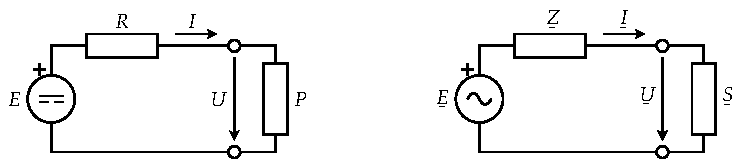
\includegraphics{Imatges/Cap-CalcBas-EZS.pdf}
    \captionof{figure}{Resoluci\'{o} de circuits coneixent la pot\`{e}ncia absorbida per la c\`{a}rrega} \label{pic:EZS}
\end{center}

\subsection{Circuits de corrent continu}

A partir del circuit de l'esquerra de la Figura \vref{pic:EZS} tenim les dues equacions seg\"{u}ents:
\begin{align}
   E &= R I + U \label{eq:ERP_1} \\
   P &= U I     \label{eq:ERP_2}
\end{align}

Multiplicant l'equaci\'{o} \eqref{eq:ERP_1} per $U$ i substituint l'equaci\'{o} \eqref{eq:ERP_2} en aquest resultat, tenim:
\begin{equation}
   E U = R I U + U^2 = R P + U^2 \quad \rightarrow \quad U^2 - E U + R P = 0 \label{eq:ERP_3}
\end{equation}

A partir de les equacions descrites anteriorment, el circuit es resol seguint els seg\"{u}ents passos:
\begin{dingautolist}{'312}
   \item Obtenim $U$, resolent l'equaci\'{o} de 2n grau \eqref{eq:ERP_3}.
   \item Dels dos valors reals que obtenim, ens quedem amb el m\'{e}s elevat. Si en lloc de dos valors reals, obtingu\'{e}ssim
   un parell de valors conjugats complexos, aix\`{o} ens indicaria que el circuit no t\'{e} una soluci\'{o} f\'{\i}sicament possible, i per tant no seria resoluble.
   \item Finalment, calculem $I$ substituint el valor trobat de $U$ en l'equaci\'{o} \eqref{eq:ERP_2}.
\end{dingautolist}

Un cop trobats $U$ i $I$, podem calcular el valor de la resist\`{e}ncia
$R\ped{P}$ de la c\`{a}rrega, la qual absorbeix la pot\`{e}ncia $P$, a
partir de l'equaci\'{o} \eqref{eq:ERP_2} i de la relaci\'{o} $U =R\ped{P}
I$:
\begin{equation}
   R\ped{P} = \frac{U}{I} = \frac{P}{I^2} = \frac{U^2}{P}
\end{equation}

\subsection{Circuits de corrent altern}

A partir del circuit de la dreta de la Figura \vref{pic:EZS} tenim les dues equacions seg\"{u}ents:
\begin{align}
   \cmplx{E} &= \cmplx{Z} \, \cmplx{I} + \cmplx{U} \label{eq:EZS_1} \\
   \cmplx{S} &= \cmplx{U} \, \cmplx{I}^*           \label{eq:EZS_2}
\end{align}

Conjugant l'equaci\'{o} \eqref{eq:EZS_1}, multiplicant-la per $\cmplx{U}$ i substituint l'equaci\'{o} \eqref{eq:EZS_2} en aquest resultat, tenim:
\begin{equation}
   \cmplx{E}^* \, \cmplx{U} = \cmplx{Z}^* \cmplx{I}^* \, \cmplx{U} + \cmplx{U}^* \, \cmplx{U} =
   \cmplx{Z}^* \, \cmplx{S} + |\cmplx{U}|^2 \quad \rightarrow \quad
   |\cmplx{U}|^2 - \cmplx{E}^* \, \cmplx{U} + \cmplx{Z}^* \, \cmplx{S} = 0
   \label{eq:EZS_3}
\end{equation}

Fem a continuaci\'{o} una rotaci\'{o} dels fasors $\cmplx{E}$ i
$\cmplx{U}$, de valor $\eu^{-\ju\psi}$, on $\psi$ \'{e}s l'argument
del fasor $\cmplx{E}$; d'aquesta manera, el nou fasor $E'$ tan
sols tindr\`{a} part real, i el nou fasor $\cmplx{U}'$ estar\`{a} rotat
respecte del fasor $\cmplx{U}$.
\begin{align}
   \psi &= \arg(\cmplx{E}) \label{eq:EZS_9} \\
   E' &= \cmplx{E} \, \eu^{-\ju\psi} = |\cmplx{E}|  \label{eq:EZS_4} \\
   \cmplx{U}' &= \cmplx{U} \, \eu^{-\ju\psi}   \label{eq:EZS_5}
\end{align}

Expressem a continuaci\'{o} l'equaci\'{o} \eqref{eq:EZS_3} utilitzant
aquests dos nous fasors:
\begin{equation}
   |\cmplx{U}'|^2 - E' \, \cmplx{U}' + \cmplx{Z}^* \, \cmplx{S} = 0 \label{eq:EZS_6}
\end{equation}

Finalment, separem l'equaci\'{o} \eqref{eq:EZS_6} en dues, una per a la part real i una altra per a la part imagin\`{a}ria. Cal tenir en compte que $|\cmplx{U}'|^2$ nom\'{e}s t\'{e} part real, de valor $\Re^2(\cmplx{U}') + \Im^2(\cmplx{U}')$.
\begin{align}
   \Re^2(\cmplx{U}') + \Im^2(\cmplx{U}') - E' \, \Re(\cmplx{U}') + \Re(\cmplx{Z}^* \, \cmplx{S}) &= 0 \label{eq:EZS_7} \\
   - E' \, \Im(\cmplx{U}') + \Im(\cmplx{Z}^* \, \cmplx{S}) &= 0 \label{eq:EZS_8}
\end{align}

A partir de les equacions descrites anteriorment, el circuit es resol seguint els seg\"{u}ents passos:
\begin{dingautolist}{'312}
   \item Calculem $E'$ a partir de l'equaci\'{o} \eqref{eq:EZS_4}
   \item Obtenim $\Im(\cmplx{U}')$, resolent l'equaci\'{o} \eqref{eq:EZS_8}.
   \item Substitu\"{\i}m el valor obtingut per a $\Im(\cmplx{U}')$ en l'equaci\'{o} \eqref{eq:EZS_7}, i obtenim $\Re(\cmplx{U}')$ resolent aquesta equaci\'{o} de 2n grau.
   \item Dels dos valors reals que obtenim, ens quedem amb el m\'{e}s elevat. Si en lloc de dos valors reals, obtingu\'{e}ssim un parell de valors conjugats complexos, aix\`{o} ens indicaria que el circuit no t\'{e} una soluci\'{o} f\'{\i}sicament possible, i per tant no seria resoluble.
   \item A partir del valor  obtingut per a $\cmplx{U}'$ en el passos anteriors, i del valor de $\psi$ obtingut a partir de l'equaci\'{o} \eqref{eq:EZS_9}, calculem el valor buscat de $\cmplx{U}$, utilitzant l'equaci\'{o} \eqref{eq:EZS_5}
   \item Finalment, calculem $\cmplx{I}$ substituint el valor trobat de $\cmplx{U}$ en l'equaci\'{o} \eqref{eq:EZS_2}
\end{dingautolist}

Un cop trobats $\cmplx{U}$ i $\cmplx{I}$, podem calcular el valor de
la imped\`{a}ncia  $\cmplx{Z}\ped{S}$ de la c\`{a}rrega, la qual absorbeix
la pot\`{e}ncia $\cmplx{S}$, a partir de l'equaci\'{o} \eqref{eq:EZS_2} i de
la relaci\'{o} $\cmplx{U} = \cmplx{Z}\ped{S} \,\cmplx{I}$:

\begin{equation}
   \cmplx{Z}\ped{S} = \frac{\cmplx{U}}{\cmplx{I}} =
   \frac{\cmplx{S}}{|\cmplx{I}|^2} =
   \frac{|\cmplx{U}|^2}{\cmplx{S}^*} \label{eq:EZS 10}
\end{equation}

\begin{exemple}[Resoluci\'{o} d'un circuit coneixent la pot\`{e}ncia que absorbeix]
    Resoldre el circuit de la dreta de la Figura \vref{pic:EZS}, donats el seg\"{u}ents valors en per unitat:

    \[
       \cmplx{E} = \num{0,4 + j 0,3} \qquad \cmplx{Z} = \num{j 0,1} \qquad
       \cmplx{S} = \num{0,6 + j 0,45}
    \]

    Calculem primer $\psi$ i $E'$, segons les equacions \eqref{eq:EZS_9} i \eqref{eq:EZS_4},
    i $\cmplx{Z}^* \cmplx{S}$:

    \begin{align*}
       \psi &= \arg(\num{0,4 + j 0,3}) = \SI{0,6435}{rad} \\
       E' &= |\num{0,4 + j 0,3}| = \num {0,5} \\
       \cmplx{Z}^* \cmplx{S} &= \num{- j 0,1} \times (\num{0,6 + j 0,45}) = \num{0,045 - j 0,06}
    \end{align*}

    Calculem a continuaci\'{o} $\Im(\cmplx{U}')$, segons l'equaci\'{o} \eqref{eq:EZS_8}:

    \[
       \Im(\cmplx{U}') = \frac{\Im(\cmplx{Z}^* \cmplx{S})}{E'} = \frac{\num{-0,06}}{\num{0,5}} = \num{-0,12}
    \]

    Formem a continuaci\'{o} el polinomi de 2n grau en $\Re(\cmplx{U}')$ i el resolem, segons l'equaci\'{o} \eqref{eq:EZS_7}:

    \begin{align*}
       \Re^2(\cmplx{U}') + (\num{-0,12})^2 - \num{0,5} \times \Re(\cmplx{U}') + \num{0,045} &= 0 \\
       \Re^2(\cmplx{U}') - \num{0,5} \times \Re(\cmplx{U}') + \num{0,0594} &= 0  \;\rightarrow\; \Re(\cmplx{U}') =
       \left\{ \begin{matrix}
         \num{0,1943} \\
         \boxed{\num{0,3057}}
       \end{matrix}
       \right.
    \end{align*}

    Prenent el valor m\'{e}s elevat de $\Re(\cmplx{U}')$ calculem finalment $\cmplx{U}$, segons l'equaci\'{o} \eqref{eq:EZS_5}:

    \[
       \cmplx{U} = \cmplx{U}' \, \eu^{\ju \psi} = (\num{0,3057 - j 0,12}) \times \eu^{\num{j 0,6435}} =
       \num{0,3165 + j 0,0874}
    \]

    Obtenim ara $\cmplx{I}$, segons l'equaci\'{o} \eqref{eq:EZS_2}:

    \[
       \cmplx{I} = \frac{\cmplx{S}^*}{\cmplx{U}^*} = \frac{\num{0,6-j 0,45}}{\num{0,3165 - j 0,0874}}
       = \num{2,1262 - j 0,8347}
    \]

    Per acabar, calculem $\cmplx{Z}\ped{S}$, segons l'equaci\'{o}
    \eqref{eq:EZS 10}:

    \[
        \cmplx{Z}\ped{S} = \frac{\cmplx{U}}{\cmplx{I}} = \frac{\num{0,3165 + j 0,0874}}
        {\num{2,1262 - j 0,8347}} = \num{0,1150 + j 0,0863}
    \]
\end{exemple}




\section{Corrent de curtcircuit en el  secundari d'un transformador}
\index{corrent de curtcircuit!en el  secundari d'un transformador}

 Es tracta en aquest apartat, el c\`{a}lcul del corrent de curtcircuit trif\`{a}sic en el secundari d'un transformador, que t\'{e} el
primari connectat  a una xarxa de pot\`{e}ncia.

A partir de la Figura \vref{pic:cc_sec_trafo}, es tracta de trobar
el valor del corrent de curtcircuit trif\`{a}sic $I\ped{F}$ en el punt
F, essent la resta de par\`{a}metres valors coneguts.

\begin{center}
    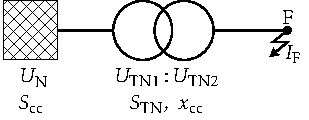
\includegraphics{Imatges/Cap-CalcBas-Icc-Trafo.pdf}
    \captionof{figure}{Corrent de curtcircuit en el  secundari d'un
transformador} \label{pic:cc_sec_trafo}
\end{center}

$U\ped{N}$, $U\ped{TN1}$ i $U\ped{TN2}$ estan donats en volt,
$S\ped{cc}$ i $S\ped{TN}$ en volt ampere, i $x\ped{cc}$ en per unitat
respecte dels valors nominals del transformador.


Per tal de simplificar el problema, suposarem que tant la imped\`{a}ncia
de curtcircuit del transformador com la imped\`{a}ncia equivalent de
la xarxa de pot\`{e}ncia s\'{o}n totalment inductives; d'aquesta manera,
podrem treballar amb les diverses variables implicades com si
fossin nombres reals. Suposarem a m\'{e}s que no hi ha circulaci\'{o} de
corrent abans del curtcircuit.

Pel que fa a la xarxa de pot\`{e}ncia, si en lloc de la pot\`{e}ncia de curtcircuit $S\ped{cc}$, el que coneixem \'{e}s el corrent de curtcircuit
disponible $I\ped{cc}$, podem obtenir el valor de la pot\`{e}ncia de
curtcircuit a partir de l'expressi\'{o}:

\begin{equation}
    S\ped{cc} = \sqrt{3} U\ped{N} I\ped{cc}
\end{equation}
\index{pot\`{e}ncia de curtcircuit}

 Si prenem com a valors base els
par\`{a}metres del transformador ($U\ped{TN1}$, $U\ped{TN2}$ i
$S\ped{TN}$), la relaci\'{o} de transformaci\'{o} i la imped\`{a}ncia de curtcircuit del transformador, expressats en per unitat, seran 1:1 i
$x\ped{cc}$ respectivament. An\`{a}logament, la tensi\'{o} i la imped\`{a}ncia
equivalents de la xarxa de pot\`{e}ncia, expressats en per unitat, seran
$\frac{U\ped{N}}{U\ped{TN1}}$ i $\frac{U\ped{N}^2}{S\ped{cc}}
\frac{S\ped{TN}}{U\ped{TN1}^2}$ respectivament.

Amb aquests valors, el corrent de curtcircuit $i\ped{F}$, expressat
en per unitat, val:

\begin{equation}
    i\ped{F} = \frac{\dfrac{U\ped{N}}{U\ped{TN1}}}{\dfrac{U\ped{N}^2}{S\ped{cc}}
    \dfrac{S\ped{TN}}{U\ped{TN1}^2} + x\ped{cc}}
\end{equation}

I per tant, aquest corrent $I\ped{F}$, expressat en ampere, val:

\begin{equation}
    I\ped{F} = i\ped{F}\; \frac{S\ped{TN}}{\sqrt{3}U\ped{TN2}} =
    \frac{S\ped{TN} U\ped{N}}{\sqrt{3} U\ped{TN1}U\ped{TN2}
    \left(\dfrac{U\ped{N}^2}{S\ped{cc}}
    \dfrac{S\ped{TN}}{U\ped{TN1}^2} + x\ped{cc}\right)}
\end{equation}

Si la xarxa de pot\`{e}ncia es considera de pot\`{e}ncia infinita, tenim:

\begin{equation}
    I\ped{F} = \frac{S\ped{TN} U\ped{N}}{\sqrt{3} U\ped{TN1}U\ped{TN2}
    x\ped{cc}}\qquad\qquad (\text{amb }S\ped{cc}=\infty)
\end{equation}

Si a m\'{e}s, la tensi\'{o} de la xarxa coincideix amb la tensi\'{o} prim\`{a}ria
del transformador, tenim respectivament:

\begin{align}
    I\ped{F} &= \frac{S\ped{TN}}{\sqrt{3} U\ped{TN2}
    \left(\dfrac{S\ped{TN}}{S\ped{cc}} +
    x\ped{cc}\right)}\qquad\qquad(\text{amb }U\ped{N}=U\ped{TN1})\\[1ex]
    I\ped{F} &= \frac{S\ped{TN}}{\sqrt{3} U\ped{TN2}
    x\ped{cc}}\qquad\qquad(\text{amb }U\ped{N}=U\ped{TN1}\text{ i }
    S\ped{cc}=\infty)
\end{align}

\begin{exemple}[Corrent de curtcircuit en el secundari d'un transformador]
    A partir de la Figura \vref{pic:cc_sec_trafo}, amb els valors
    $U\ped{N}=\SI{6900}{V}$, $U\ped{TN1}=\SI{6900}{V}$,
    $U\ped{TN2}=\SI{400}{V}$, $S\ped{TN}=\SI{850}{kVA}$ i
    $x\ped{cc}=\SI{5}{\%}$, es tracta de trobar $I\ped{F}$ en el cas
    que: a) $S\ped{cc}=\SI{200}{MVA}$ i b) $S\ped{cc}=\infty$.

    El valors demanats s\'{o}n:

    \begin{align*}
       &a)\;I\ped{F} = \frac{\SI{850}{kVA}}{\sqrt{3}\times \SI{400}{V}\times
       \left(\dfrac{\SI{850}{kVA}}{\SI{200}{MVA}} +
       \num{0,05}\right)} = \SI{22,6}{kA} \\[1ex]
       &b)\;I\ped{F} = \frac{\SI{850}{kVA}}{\sqrt{3}\times \SI{400}{V}\times
       \num{0,05}} = \SI{24,5}{kA}
    \end{align*}
\end{exemple}




\section{Escales logar\'{\i}tmiques} \index{escales logar\'{\i}tmiques}

En diferents camps de l'electrot\`{e}cnia \'{e}s usual trobar-se gr\`{a}fics amb escales
logar\'{\i}tmiques.

Un exemple clar s\'{o}n els gr\`{a}fics d'actuaci\'{o} dels interruptors magnetot\`{e}rmics o dels
fusibles, on les seves corbes caracter\'{\i}stiques corrent--temps estan representades en
una escala logar\'{\i}tmica--logar\'{\i}tmica o lineal--logar\'{\i}tmica.

En aquests casos es presenta freq\"{u}entment la necessitat de determinar amb exactitud un
punt de la corba, que no coincideix amb cap de les l\'{\i}nies divis\`{o}ries del gr\`{a}fic. Atenent a
la Figura \vref{pic:escala log}, es tracta de determinar el valor $x$ dins de la d\`{e}cada
$10^N$ a $10^{N+1}$.

\begin{center}
    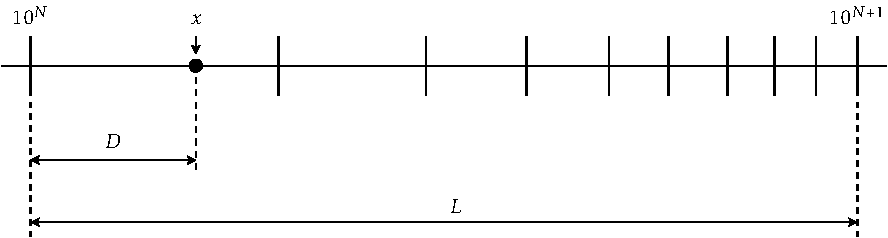
\includegraphics{Imatges/Cap-CalcBas-EscalesLog.pdf}
    \captionof{figure}{Escala logar\'{\i}tmica}
    \label{pic:escala log}
\end{center}

Si mesurem amb un regle la dist\`{a}ncia $D$ des de l'inici de la d\`{e}cada fins al punt $x$, i
la longitud total $L$ de la d\`{e}cada, el valor $x$ buscat ve donat per l'expressi\'{o}:

\begin{equation}
    x = 10^{\left(N+\frac{D}{L}\right)}
\end{equation}

Si estem interessats en el problema invers, \'{e}s a dir, en  trobar la dist\`{a}ncia $D$
corresponent a un valor conegut $x$ dins de la d\`{e}cada $10^N$ a $10^{N+1}$, podem emprar
l'expressi\'{o}:

\begin{equation}
    D = L(\log x - N) = L \log\frac{x}{10^N}
\end{equation}

\begin{exemple}[C\`{a}lcul d'un valor en una escala logar\'{\i}tmica]
    Es tracta de trobar el valor $x$ dins de la d\`{e}cada 100 a 1000, corresponent a una
    dist\`{a}ncia $D=\SI{11}{mm}$; la longitud total de la d\`{e}cada \'{e}s $L=\SI{56}{mm}$.

    En aquest cas tenim $N=2$, i per tant:
    \[
        x = 10^{\left(2+\frac{\SI{11}{mm}}{\SI{56}{mm}}\right)}= \num{157,19}
    \]
\end{exemple}

\begin{exemple}[Representaci\'{o} d'un valor en una escala logar\'{\i}tmica]
    Es tracta de trobar la dist\`{a}ncia $D$ a la qual hem de representar el valor $x=5$, dins de la
    d\`{e}cada 1 a 10; la longitud total de la d\`{e}cada \'{e}s $L=\SI{56}{mm}$.

    En aquest cas tenim $N=0$, i per tant:

    \[
        D = \SI{56}{mm} \times (\log 5 - 0)  = \SI{39,1}{mm}
    \]
\end{exemple}

